

\tikzset{every picture/.style={line width=0.75pt}} %set default line width to 0.75pt        

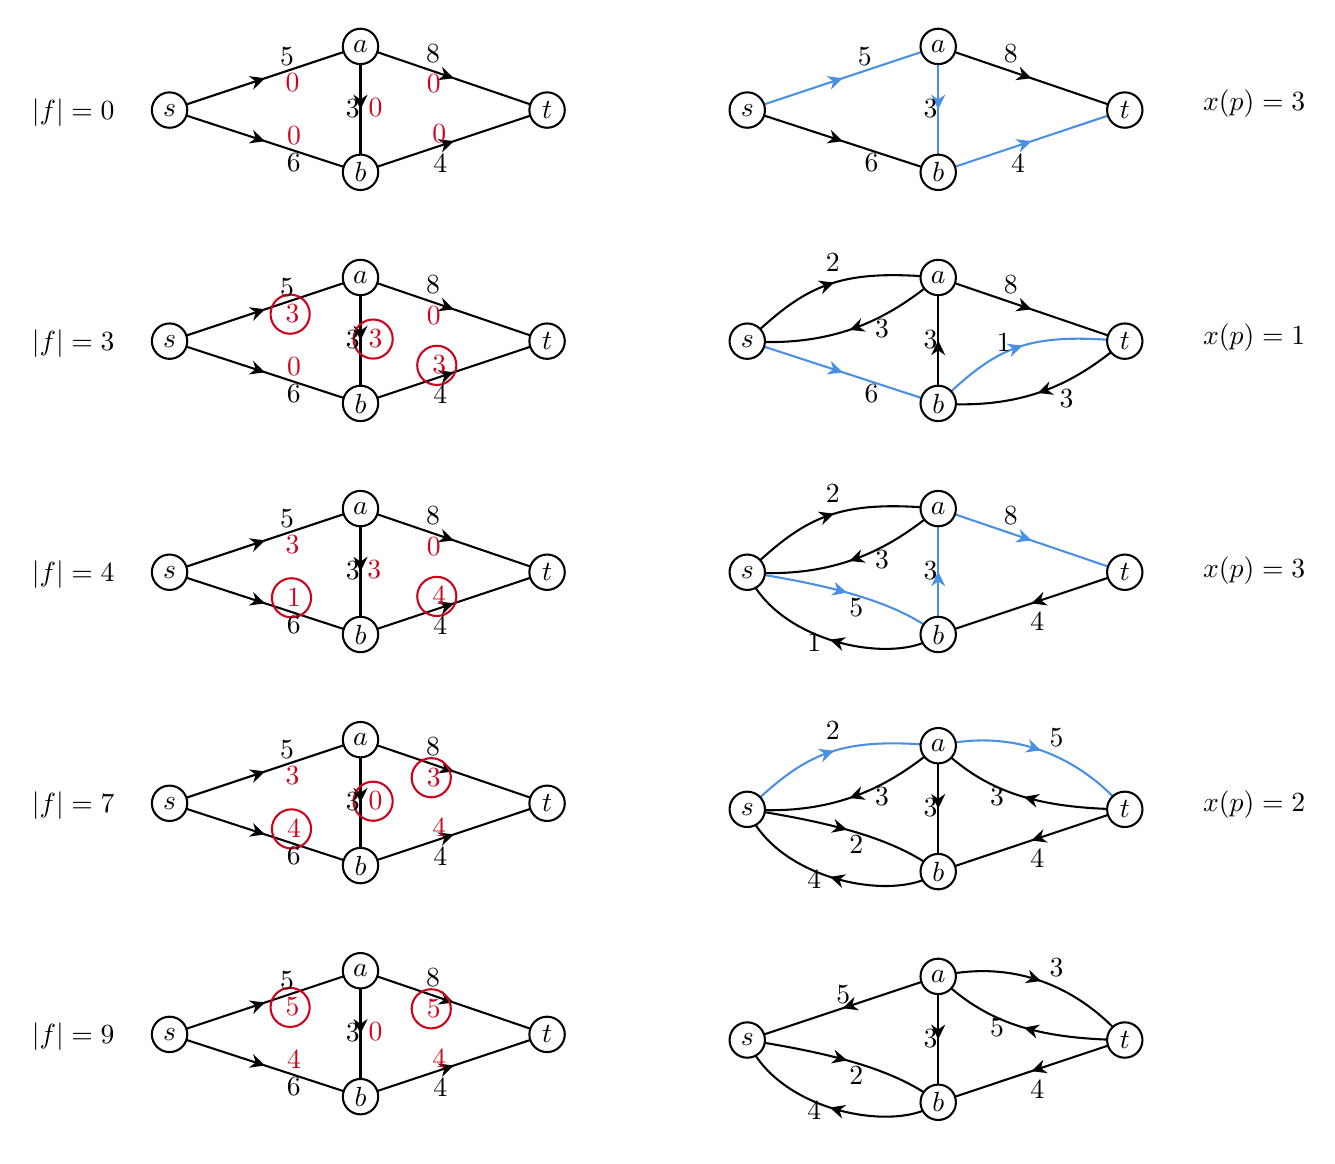
\begin{tikzpicture}[x=0.5pt,y=0.5pt,yscale=-1,xscale=1]
%uncomment if require: \path (0,839); %set diagram left start at 0, and has height of 839

%Straight Lines [id:da5712618432248621] 
\draw    (824.12,415.76) -- (689.29,460.76) ;
\draw [shift={(756.71,438.26)}, rotate = 341.53999999999996] [fill={rgb, 255:red, 0; green, 0; blue, 0 }  ][line width=0.08]  [draw opacity=0] (10.72,-5.15) -- (0,0) -- (10.72,5.15) -- (7.12,0) -- cycle    ;
%Curve Lines [id:da21939430850053032] 
\draw [color={rgb, 255:red, 74; green, 144; blue, 226 }  ,draw opacity=1 ]   (551.29,415.76) .. controls (617,426.01) and (660,438.01) .. (689.29,460.76) ;
\draw [shift={(623.46,430.47)}, rotate = 195.08] [fill={rgb, 255:red, 74; green, 144; blue, 226 }  ,fill opacity=1 ][line width=0.08]  [draw opacity=0] (10.72,-5.15) -- (0,0) -- (10.72,5.15) -- (7.12,0) -- cycle    ;
%Curve Lines [id:da15773096786649754] 
\draw    (689.29,460.76) .. controls (661,484.01) and (573,468.01) .. (551.29,415.76) ;
\draw [shift={(611.07,464.56)}, rotate = 376.76] [fill={rgb, 255:red, 0; green, 0; blue, 0 }  ][line width=0.08]  [draw opacity=0] (10.72,-5.15) -- (0,0) -- (10.72,5.15) -- (7.12,0) -- cycle    ;
%Straight Lines [id:da024680351236297304] 
\draw [color={rgb, 255:red, 74; green, 144; blue, 226 }  ,draw opacity=1 ]   (689.29,369.76) -- (824.12,415.76) ;
\draw [shift={(756.71,392.76)}, rotate = 198.84] [fill={rgb, 255:red, 74; green, 144; blue, 226 }  ,fill opacity=1 ][line width=0.08]  [draw opacity=0] (10.72,-5.15) -- (0,0) -- (10.72,5.15) -- (7.12,0) -- cycle    ;
%Curve Lines [id:da14623738071334857] 
\draw    (551.29,415.76) .. controls (593,376.01) and (616,363.01) .. (689.29,369.76) ;
\draw [shift={(613.98,373.47)}, rotate = 521.52] [fill={rgb, 255:red, 0; green, 0; blue, 0 }  ][line width=0.08]  [draw opacity=0] (10.72,-5.15) -- (0,0) -- (10.72,5.15) -- (7.12,0) -- cycle    ;
%Curve Lines [id:da1884084092202849] 
\draw    (689.29,369.76) .. controls (661,393.01) and (622,421.01) .. (551.29,415.76) ;
\draw [shift={(625.16,407.6)}, rotate = 340.45] [fill={rgb, 255:red, 0; green, 0; blue, 0 }  ][line width=0.08]  [draw opacity=0] (10.72,-5.15) -- (0,0) -- (10.72,5.15) -- (7.12,0) -- cycle    ;
%Straight Lines [id:da5031539886046075] 
\draw [color={rgb, 255:red, 74; green, 144; blue, 226 }  ,draw opacity=1 ]   (689.29,369.76) -- (689.29,460.76) ;
\draw [shift={(689.29,415.26)}, rotate = 90] [fill={rgb, 255:red, 74; green, 144; blue, 226 }  ,fill opacity=1 ][line width=0.08]  [draw opacity=0] (10.72,-5.15) -- (0,0) -- (10.72,5.15) -- (7.12,0) -- cycle    ;
%Shape: Ellipse [id:dp5508071293563598] 
\draw  [fill={rgb, 255:red, 255; green, 255; blue, 255 }  ,fill opacity=1 ] (538.5,415.76) .. controls (538.5,408.7) and (544.23,402.97) .. (551.29,402.97) .. controls (558.36,402.97) and (564.08,408.7) .. (564.08,415.76) .. controls (564.08,422.83) and (558.36,428.55) .. (551.29,428.55) .. controls (544.23,428.55) and (538.5,422.83) .. (538.5,415.76) -- cycle ;
%Shape: Ellipse [id:dp5972831071444443] 
\draw  [fill={rgb, 255:red, 255; green, 255; blue, 255 }  ,fill opacity=1 ] (811.33,415.76) .. controls (811.33,408.7) and (817.06,402.97) .. (824.12,402.97) .. controls (831.19,402.97) and (836.91,408.7) .. (836.91,415.76) .. controls (836.91,422.83) and (831.19,428.55) .. (824.12,428.55) .. controls (817.06,428.55) and (811.33,422.83) .. (811.33,415.76) -- cycle ;
%Shape: Ellipse [id:dp04179037888015247] 
\draw  [fill={rgb, 255:red, 255; green, 255; blue, 255 }  ,fill opacity=1 ] (676.5,369.76) .. controls (676.5,362.7) and (682.23,356.97) .. (689.29,356.97) .. controls (696.36,356.97) and (702.08,362.7) .. (702.08,369.76) .. controls (702.08,376.83) and (696.36,382.55) .. (689.29,382.55) .. controls (682.23,382.55) and (676.5,376.83) .. (676.5,369.76) -- cycle ;
%Shape: Ellipse [id:dp6412358417638034] 
\draw  [fill={rgb, 255:red, 255; green, 255; blue, 255 }  ,fill opacity=1 ] (676.5,460.76) .. controls (676.5,453.7) and (682.23,447.97) .. (689.29,447.97) .. controls (696.36,447.97) and (702.08,453.7) .. (702.08,460.76) .. controls (702.08,467.83) and (696.36,473.55) .. (689.29,473.55) .. controls (682.23,473.55) and (676.5,467.83) .. (676.5,460.76) -- cycle ;

%Straight Lines [id:da7930208884666833] 
\draw    (824.12,587.12) -- (689.29,632.12) ;
\draw [shift={(756.71,609.62)}, rotate = 341.53999999999996] [fill={rgb, 255:red, 0; green, 0; blue, 0 }  ][line width=0.08]  [draw opacity=0] (10.72,-5.15) -- (0,0) -- (10.72,5.15) -- (7.12,0) -- cycle    ;
%Curve Lines [id:da7926875310432893] 
\draw [color={rgb, 255:red, 74; green, 144; blue, 226 }  ,draw opacity=1 ]   (689.29,541.12) .. controls (753,526.36) and (799,557.36) .. (824.12,587.12) ;
\draw [shift={(763.54,544.46)}, rotate = 198.02] [fill={rgb, 255:red, 74; green, 144; blue, 226 }  ,fill opacity=1 ][line width=0.08]  [draw opacity=0] (10.72,-5.15) -- (0,0) -- (10.72,5.15) -- (7.12,0) -- cycle    ;
%Curve Lines [id:da34610507417952074] 
\draw    (824.12,587.12) .. controls (760,586.36) and (723,574.36) .. (689.29,541.12) ;
\draw [shift={(751.2,578.16)}, rotate = 375.31] [fill={rgb, 255:red, 0; green, 0; blue, 0 }  ][line width=0.08]  [draw opacity=0] (10.72,-5.15) -- (0,0) -- (10.72,5.15) -- (7.12,0) -- cycle    ;
%Curve Lines [id:da11719531956200613] 
\draw [color={rgb, 255:red, 0; green, 0; blue, 0 }  ,draw opacity=1 ]   (551.29,587.12) .. controls (617,597.36) and (660,609.36) .. (689.29,632.12) ;
\draw [shift={(623.46,601.82)}, rotate = 195.08] [fill={rgb, 255:red, 0; green, 0; blue, 0 }  ,fill opacity=1 ][line width=0.08]  [draw opacity=0] (10.72,-5.15) -- (0,0) -- (10.72,5.15) -- (7.12,0) -- cycle    ;
%Curve Lines [id:da7905174995974347] 
\draw    (689.29,632.12) .. controls (661,655.36) and (573,639.36) .. (551.29,587.12) ;
\draw [shift={(611.07,635.92)}, rotate = 376.76] [fill={rgb, 255:red, 0; green, 0; blue, 0 }  ][line width=0.08]  [draw opacity=0] (10.72,-5.15) -- (0,0) -- (10.72,5.15) -- (7.12,0) -- cycle    ;
%Curve Lines [id:da9600867922426221] 
\draw [color={rgb, 255:red, 74; green, 144; blue, 226 }  ,draw opacity=1 ]   (551.29,587.12) .. controls (593,547.36) and (616,534.36) .. (689.29,541.12) ;
\draw [shift={(613.98,544.83)}, rotate = 521.52] [fill={rgb, 255:red, 74; green, 144; blue, 226 }  ,fill opacity=1 ][line width=0.08]  [draw opacity=0] (10.72,-5.15) -- (0,0) -- (10.72,5.15) -- (7.12,0) -- cycle    ;
%Curve Lines [id:da13291256320284295] 
\draw    (689.29,541.12) .. controls (661,564.36) and (622,592.36) .. (551.29,587.12) ;
\draw [shift={(625.16,578.95)}, rotate = 340.45] [fill={rgb, 255:red, 0; green, 0; blue, 0 }  ][line width=0.08]  [draw opacity=0] (10.72,-5.15) -- (0,0) -- (10.72,5.15) -- (7.12,0) -- cycle    ;
%Straight Lines [id:da930573142722233] 
\draw [color={rgb, 255:red, 0; green, 0; blue, 0 }  ,draw opacity=1 ]   (689.29,541.12) -- (689.29,632.12) ;
\draw [shift={(689.29,586.62)}, rotate = 270] [fill={rgb, 255:red, 0; green, 0; blue, 0 }  ,fill opacity=1 ][line width=0.08]  [draw opacity=0] (10.72,-5.15) -- (0,0) -- (10.72,5.15) -- (7.12,0) -- cycle    ;
%Shape: Ellipse [id:dp3114316528358767] 
\draw  [fill={rgb, 255:red, 255; green, 255; blue, 255 }  ,fill opacity=1 ] (538.5,587.12) .. controls (538.5,580.05) and (544.23,574.33) .. (551.29,574.33) .. controls (558.36,574.33) and (564.08,580.05) .. (564.08,587.12) .. controls (564.08,594.18) and (558.36,599.91) .. (551.29,599.91) .. controls (544.23,599.91) and (538.5,594.18) .. (538.5,587.12) -- cycle ;
%Shape: Ellipse [id:dp3160104397757745] 
\draw  [fill={rgb, 255:red, 255; green, 255; blue, 255 }  ,fill opacity=1 ] (811.33,587.12) .. controls (811.33,580.05) and (817.06,574.33) .. (824.12,574.33) .. controls (831.19,574.33) and (836.91,580.05) .. (836.91,587.12) .. controls (836.91,594.18) and (831.19,599.91) .. (824.12,599.91) .. controls (817.06,599.91) and (811.33,594.18) .. (811.33,587.12) -- cycle ;
%Shape: Ellipse [id:dp046207551745677256] 
\draw  [fill={rgb, 255:red, 255; green, 255; blue, 255 }  ,fill opacity=1 ] (676.5,541.12) .. controls (676.5,534.05) and (682.23,528.33) .. (689.29,528.33) .. controls (696.36,528.33) and (702.08,534.05) .. (702.08,541.12) .. controls (702.08,548.18) and (696.36,553.91) .. (689.29,553.91) .. controls (682.23,553.91) and (676.5,548.18) .. (676.5,541.12) -- cycle ;
%Shape: Ellipse [id:dp3969469730815376] 
\draw  [fill={rgb, 255:red, 255; green, 255; blue, 255 }  ,fill opacity=1 ] (676.5,632.12) .. controls (676.5,625.05) and (682.23,619.33) .. (689.29,619.33) .. controls (696.36,619.33) and (702.08,625.05) .. (702.08,632.12) .. controls (702.08,639.18) and (696.36,644.91) .. (689.29,644.91) .. controls (682.23,644.91) and (676.5,639.18) .. (676.5,632.12) -- cycle ;

%Straight Lines [id:da49158415758891016] 
\draw    (824.12,753.83) -- (689.29,798.83) ;
\draw [shift={(756.71,776.33)}, rotate = 341.53999999999996] [fill={rgb, 255:red, 0; green, 0; blue, 0 }  ][line width=0.08]  [draw opacity=0] (10.72,-5.15) -- (0,0) -- (10.72,5.15) -- (7.12,0) -- cycle    ;
%Straight Lines [id:da28860157747304216] 
\draw [color={rgb, 255:red, 0; green, 0; blue, 0 }  ,draw opacity=1 ]   (689.29,707.83) -- (551.29,753.83) ;
\draw [shift={(620.29,730.83)}, rotate = 341.57] [fill={rgb, 255:red, 0; green, 0; blue, 0 }  ,fill opacity=1 ][line width=0.08]  [draw opacity=0] (10.72,-5.15) -- (0,0) -- (10.72,5.15) -- (7.12,0) -- cycle    ;
%Curve Lines [id:da15178288365573256] 
\draw [color={rgb, 255:red, 0; green, 0; blue, 0 }  ,draw opacity=1 ]   (689.29,707.83) .. controls (753,693.07) and (799,724.07) .. (824.12,753.83) ;
\draw [shift={(763.54,711.17)}, rotate = 198.02] [fill={rgb, 255:red, 0; green, 0; blue, 0 }  ,fill opacity=1 ][line width=0.08]  [draw opacity=0] (10.72,-5.15) -- (0,0) -- (10.72,5.15) -- (7.12,0) -- cycle    ;
%Curve Lines [id:da3540522280257019] 
\draw    (824.12,753.83) .. controls (760,753.07) and (723,741.07) .. (689.29,707.83) ;
\draw [shift={(751.2,744.87)}, rotate = 375.31] [fill={rgb, 255:red, 0; green, 0; blue, 0 }  ][line width=0.08]  [draw opacity=0] (10.72,-5.15) -- (0,0) -- (10.72,5.15) -- (7.12,0) -- cycle    ;
%Curve Lines [id:da060897532886768135] 
\draw [color={rgb, 255:red, 0; green, 0; blue, 0 }  ,draw opacity=1 ]   (551.29,753.83) .. controls (617,764.07) and (660,776.07) .. (689.29,798.83) ;
\draw [shift={(623.46,768.53)}, rotate = 195.08] [fill={rgb, 255:red, 0; green, 0; blue, 0 }  ,fill opacity=1 ][line width=0.08]  [draw opacity=0] (10.72,-5.15) -- (0,0) -- (10.72,5.15) -- (7.12,0) -- cycle    ;
%Curve Lines [id:da786245575835992] 
\draw    (689.29,798.83) .. controls (661,822.07) and (573,806.07) .. (551.29,753.83) ;
\draw [shift={(611.07,802.63)}, rotate = 376.76] [fill={rgb, 255:red, 0; green, 0; blue, 0 }  ][line width=0.08]  [draw opacity=0] (10.72,-5.15) -- (0,0) -- (10.72,5.15) -- (7.12,0) -- cycle    ;
%Straight Lines [id:da44093867915119234] 
\draw [color={rgb, 255:red, 0; green, 0; blue, 0 }  ,draw opacity=1 ]   (689.29,707.83) -- (689.29,798.83) ;
\draw [shift={(689.29,753.33)}, rotate = 270] [fill={rgb, 255:red, 0; green, 0; blue, 0 }  ,fill opacity=1 ][line width=0.08]  [draw opacity=0] (10.72,-5.15) -- (0,0) -- (10.72,5.15) -- (7.12,0) -- cycle    ;
%Shape: Ellipse [id:dp7083364570909119] 
\draw  [fill={rgb, 255:red, 255; green, 255; blue, 255 }  ,fill opacity=1 ] (538.5,753.83) .. controls (538.5,746.76) and (544.23,741.04) .. (551.29,741.04) .. controls (558.36,741.04) and (564.08,746.76) .. (564.08,753.83) .. controls (564.08,760.89) and (558.36,766.62) .. (551.29,766.62) .. controls (544.23,766.62) and (538.5,760.89) .. (538.5,753.83) -- cycle ;
%Shape: Ellipse [id:dp9011154955575111] 
\draw  [fill={rgb, 255:red, 255; green, 255; blue, 255 }  ,fill opacity=1 ] (811.33,753.83) .. controls (811.33,746.76) and (817.06,741.04) .. (824.12,741.04) .. controls (831.19,741.04) and (836.91,746.76) .. (836.91,753.83) .. controls (836.91,760.89) and (831.19,766.62) .. (824.12,766.62) .. controls (817.06,766.62) and (811.33,760.89) .. (811.33,753.83) -- cycle ;
%Shape: Ellipse [id:dp13631823330208592] 
\draw  [fill={rgb, 255:red, 255; green, 255; blue, 255 }  ,fill opacity=1 ] (676.5,707.83) .. controls (676.5,700.76) and (682.23,695.04) .. (689.29,695.04) .. controls (696.36,695.04) and (702.08,700.76) .. (702.08,707.83) .. controls (702.08,714.89) and (696.36,720.62) .. (689.29,720.62) .. controls (682.23,720.62) and (676.5,714.89) .. (676.5,707.83) -- cycle ;
%Shape: Ellipse [id:dp5722233383669696] 
\draw  [fill={rgb, 255:red, 255; green, 255; blue, 255 }  ,fill opacity=1 ] (676.5,798.83) .. controls (676.5,791.76) and (682.23,786.04) .. (689.29,786.04) .. controls (696.36,786.04) and (702.08,791.76) .. (702.08,798.83) .. controls (702.08,805.89) and (696.36,811.62) .. (689.29,811.62) .. controls (682.23,811.62) and (676.5,805.89) .. (676.5,798.83) -- cycle ;

%Straight Lines [id:da5046319954769127] 
\draw    (689.29,202.76) -- (824.12,248.76) ;
\draw [shift={(756.71,225.76)}, rotate = 198.84] [fill={rgb, 255:red, 0; green, 0; blue, 0 }  ][line width=0.08]  [draw opacity=0] (10.72,-5.15) -- (0,0) -- (10.72,5.15) -- (7.12,0) -- cycle    ;
%Curve Lines [id:da38278639324563646] 
\draw [color={rgb, 255:red, 74; green, 144; blue, 226 }  ,draw opacity=1 ]   (689.29,293.76) .. controls (731,254.01) and (750.83,242.01) .. (824.12,248.76) ;
\draw [shift={(750.19,252.04)}, rotate = 521.48] [fill={rgb, 255:red, 74; green, 144; blue, 226 }  ,fill opacity=1 ][line width=0.08]  [draw opacity=0] (10.72,-5.15) -- (0,0) -- (10.72,5.15) -- (7.12,0) -- cycle    ;
%Curve Lines [id:da1766104925762454] 
\draw    (824.12,248.76) .. controls (795.83,272.01) and (760,299.01) .. (689.29,293.76) ;
\draw [shift={(761.26,286.2)}, rotate = 340.65] [fill={rgb, 255:red, 0; green, 0; blue, 0 }  ][line width=0.08]  [draw opacity=0] (10.72,-5.15) -- (0,0) -- (10.72,5.15) -- (7.12,0) -- cycle    ;
%Curve Lines [id:da7953750592390111] 
\draw    (551.29,248.76) .. controls (593,209.01) and (616,196.01) .. (689.29,202.76) ;
\draw [shift={(613.98,206.47)}, rotate = 521.52] [fill={rgb, 255:red, 0; green, 0; blue, 0 }  ][line width=0.08]  [draw opacity=0] (10.72,-5.15) -- (0,0) -- (10.72,5.15) -- (7.12,0) -- cycle    ;
%Curve Lines [id:da8624832393405886] 
\draw    (689.29,202.76) .. controls (661,226.01) and (622,254.01) .. (551.29,248.76) ;
\draw [shift={(625.16,240.59)}, rotate = 340.45] [fill={rgb, 255:red, 0; green, 0; blue, 0 }  ][line width=0.08]  [draw opacity=0] (10.72,-5.15) -- (0,0) -- (10.72,5.15) -- (7.12,0) -- cycle    ;
%Straight Lines [id:da6698279771979019] 
\draw [color={rgb, 255:red, 74; green, 144; blue, 226 }  ,draw opacity=1 ]   (551.29,248.76) -- (689.29,293.76) ;
\draw [shift={(620.29,271.26)}, rotate = 198.06] [fill={rgb, 255:red, 74; green, 144; blue, 226 }  ,fill opacity=1 ][line width=0.08]  [draw opacity=0] (10.72,-5.15) -- (0,0) -- (10.72,5.15) -- (7.12,0) -- cycle    ;
%Straight Lines [id:da11415001597543806] 
\draw    (689.29,202.76) -- (689.29,293.76) ;
\draw [shift={(689.29,248.26)}, rotate = 90] [fill={rgb, 255:red, 0; green, 0; blue, 0 }  ][line width=0.08]  [draw opacity=0] (10.72,-5.15) -- (0,0) -- (10.72,5.15) -- (7.12,0) -- cycle    ;
%Shape: Ellipse [id:dp40258634523399217] 
\draw  [fill={rgb, 255:red, 255; green, 255; blue, 255 }  ,fill opacity=1 ] (538.5,248.76) .. controls (538.5,241.69) and (544.23,235.97) .. (551.29,235.97) .. controls (558.36,235.97) and (564.08,241.69) .. (564.08,248.76) .. controls (564.08,255.82) and (558.36,261.55) .. (551.29,261.55) .. controls (544.23,261.55) and (538.5,255.82) .. (538.5,248.76) -- cycle ;
%Shape: Ellipse [id:dp9918043056808712] 
\draw  [fill={rgb, 255:red, 255; green, 255; blue, 255 }  ,fill opacity=1 ] (811.33,248.76) .. controls (811.33,241.69) and (817.06,235.97) .. (824.12,235.97) .. controls (831.19,235.97) and (836.91,241.69) .. (836.91,248.76) .. controls (836.91,255.82) and (831.19,261.55) .. (824.12,261.55) .. controls (817.06,261.55) and (811.33,255.82) .. (811.33,248.76) -- cycle ;
%Shape: Ellipse [id:dp9667431813629475] 
\draw  [fill={rgb, 255:red, 255; green, 255; blue, 255 }  ,fill opacity=1 ] (676.5,202.76) .. controls (676.5,195.69) and (682.23,189.97) .. (689.29,189.97) .. controls (696.36,189.97) and (702.08,195.69) .. (702.08,202.76) .. controls (702.08,209.82) and (696.36,215.55) .. (689.29,215.55) .. controls (682.23,215.55) and (676.5,209.82) .. (676.5,202.76) -- cycle ;
%Shape: Ellipse [id:dp5759426974051695] 
\draw  [fill={rgb, 255:red, 255; green, 255; blue, 255 }  ,fill opacity=1 ] (676.5,293.76) .. controls (676.5,286.69) and (682.23,280.97) .. (689.29,280.97) .. controls (696.36,280.97) and (702.08,286.69) .. (702.08,293.76) .. controls (702.08,300.82) and (696.36,306.55) .. (689.29,306.55) .. controls (682.23,306.55) and (676.5,300.82) .. (676.5,293.76) -- cycle ;

%Straight Lines [id:da6310436372388507] 
\draw    (133.79,81.75) -- (271.79,126.75) ;
\draw [shift={(202.79,104.25)}, rotate = 198.06] [fill={rgb, 255:red, 0; green, 0; blue, 0 }  ][line width=0.08]  [draw opacity=0] (10.72,-5.15) -- (0,0) -- (10.72,5.15) -- (7.12,0) -- cycle    ;
%Straight Lines [id:da9607768987146322] 
\draw    (133.79,81.75) -- (271.79,35.75) ;
\draw [shift={(202.79,58.75)}, rotate = 521.5699999999999] [fill={rgb, 255:red, 0; green, 0; blue, 0 }  ][line width=0.08]  [draw opacity=0] (10.72,-5.15) -- (0,0) -- (10.72,5.15) -- (7.12,0) -- cycle    ;
%Straight Lines [id:da5142617850685254] 
\draw    (271.79,35.75) -- (271.79,126.75) ;
\draw [shift={(271.79,81.25)}, rotate = 270] [fill={rgb, 255:red, 0; green, 0; blue, 0 }  ][line width=0.08]  [draw opacity=0] (10.72,-5.15) -- (0,0) -- (10.72,5.15) -- (7.12,0) -- cycle    ;
%Straight Lines [id:da39427162431390306] 
\draw    (271.79,35.75) -- (406.62,81.75) ;
\draw [shift={(339.21,58.75)}, rotate = 198.84] [fill={rgb, 255:red, 0; green, 0; blue, 0 }  ][line width=0.08]  [draw opacity=0] (10.72,-5.15) -- (0,0) -- (10.72,5.15) -- (7.12,0) -- cycle    ;
%Straight Lines [id:da22240625522996516] 
\draw    (271.79,126.75) -- (406.62,81.75) ;
\draw [shift={(339.21,104.25)}, rotate = 521.54] [fill={rgb, 255:red, 0; green, 0; blue, 0 }  ][line width=0.08]  [draw opacity=0] (10.72,-5.15) -- (0,0) -- (10.72,5.15) -- (7.12,0) -- cycle    ;
%Shape: Ellipse [id:dp6782142185648296] 
\draw  [fill={rgb, 255:red, 255; green, 255; blue, 255 }  ,fill opacity=1 ] (121,81.75) .. controls (121,74.69) and (126.73,68.96) .. (133.79,68.96) .. controls (140.86,68.96) and (146.58,74.69) .. (146.58,81.75) .. controls (146.58,88.82) and (140.86,94.54) .. (133.79,94.54) .. controls (126.73,94.54) and (121,88.82) .. (121,81.75) -- cycle ;
%Shape: Ellipse [id:dp3975259870386] 
\draw  [fill={rgb, 255:red, 255; green, 255; blue, 255 }  ,fill opacity=1 ] (393.83,81.75) .. controls (393.83,74.69) and (399.56,68.96) .. (406.62,68.96) .. controls (413.69,68.96) and (419.41,74.69) .. (419.41,81.75) .. controls (419.41,88.82) and (413.69,94.54) .. (406.62,94.54) .. controls (399.56,94.54) and (393.83,88.82) .. (393.83,81.75) -- cycle ;
%Shape: Ellipse [id:dp10436508901371688] 
\draw  [fill={rgb, 255:red, 255; green, 255; blue, 255 }  ,fill opacity=1 ] (259,35.75) .. controls (259,28.69) and (264.73,22.96) .. (271.79,22.96) .. controls (278.86,22.96) and (284.58,28.69) .. (284.58,35.75) .. controls (284.58,42.82) and (278.86,48.54) .. (271.79,48.54) .. controls (264.73,48.54) and (259,42.82) .. (259,35.75) -- cycle ;
%Shape: Ellipse [id:dp529081709178548] 
\draw  [fill={rgb, 255:red, 255; green, 255; blue, 255 }  ,fill opacity=1 ] (259,126.75) .. controls (259,119.69) and (264.73,113.96) .. (271.79,113.96) .. controls (278.86,113.96) and (284.58,119.69) .. (284.58,126.75) .. controls (284.58,133.82) and (278.86,139.54) .. (271.79,139.54) .. controls (264.73,139.54) and (259,133.82) .. (259,126.75) -- cycle ;

%Straight Lines [id:da9402131085035222] 
\draw    (133.79,248.75) -- (271.79,293.75) ;
\draw [shift={(202.79,271.25)}, rotate = 198.06] [fill={rgb, 255:red, 0; green, 0; blue, 0 }  ][line width=0.08]  [draw opacity=0] (10.72,-5.15) -- (0,0) -- (10.72,5.15) -- (7.12,0) -- cycle    ;
%Straight Lines [id:da5315472744817162] 
\draw    (133.79,248.75) -- (271.79,202.75) ;
\draw [shift={(202.79,225.75)}, rotate = 521.5699999999999] [fill={rgb, 255:red, 0; green, 0; blue, 0 }  ][line width=0.08]  [draw opacity=0] (10.72,-5.15) -- (0,0) -- (10.72,5.15) -- (7.12,0) -- cycle    ;
%Straight Lines [id:da31730159182207374] 
\draw    (271.79,202.75) -- (271.79,293.75) ;
\draw [shift={(271.79,248.25)}, rotate = 270] [fill={rgb, 255:red, 0; green, 0; blue, 0 }  ][line width=0.08]  [draw opacity=0] (10.72,-5.15) -- (0,0) -- (10.72,5.15) -- (7.12,0) -- cycle    ;
%Straight Lines [id:da41528232416190436] 
\draw    (271.79,202.75) -- (406.62,248.75) ;
\draw [shift={(339.21,225.75)}, rotate = 198.84] [fill={rgb, 255:red, 0; green, 0; blue, 0 }  ][line width=0.08]  [draw opacity=0] (10.72,-5.15) -- (0,0) -- (10.72,5.15) -- (7.12,0) -- cycle    ;
%Straight Lines [id:da45586904395139893] 
\draw    (271.79,293.75) -- (406.62,248.75) ;
\draw [shift={(339.21,271.25)}, rotate = 521.54] [fill={rgb, 255:red, 0; green, 0; blue, 0 }  ][line width=0.08]  [draw opacity=0] (10.72,-5.15) -- (0,0) -- (10.72,5.15) -- (7.12,0) -- cycle    ;
%Shape: Ellipse [id:dp501016284386817] 
\draw  [fill={rgb, 255:red, 255; green, 255; blue, 255 }  ,fill opacity=1 ] (121,248.75) .. controls (121,241.69) and (126.73,235.96) .. (133.79,235.96) .. controls (140.86,235.96) and (146.58,241.69) .. (146.58,248.75) .. controls (146.58,255.82) and (140.86,261.54) .. (133.79,261.54) .. controls (126.73,261.54) and (121,255.82) .. (121,248.75) -- cycle ;
%Shape: Ellipse [id:dp7538832744943658] 
\draw  [fill={rgb, 255:red, 255; green, 255; blue, 255 }  ,fill opacity=1 ] (393.83,248.75) .. controls (393.83,241.69) and (399.56,235.96) .. (406.62,235.96) .. controls (413.69,235.96) and (419.41,241.69) .. (419.41,248.75) .. controls (419.41,255.82) and (413.69,261.54) .. (406.62,261.54) .. controls (399.56,261.54) and (393.83,255.82) .. (393.83,248.75) -- cycle ;
%Shape: Ellipse [id:dp45153119663097574] 
\draw  [fill={rgb, 255:red, 255; green, 255; blue, 255 }  ,fill opacity=1 ] (259,202.75) .. controls (259,195.69) and (264.73,189.96) .. (271.79,189.96) .. controls (278.86,189.96) and (284.58,195.69) .. (284.58,202.75) .. controls (284.58,209.82) and (278.86,215.54) .. (271.79,215.54) .. controls (264.73,215.54) and (259,209.82) .. (259,202.75) -- cycle ;
%Shape: Ellipse [id:dp02663227659885714] 
\draw  [fill={rgb, 255:red, 255; green, 255; blue, 255 }  ,fill opacity=1 ] (259,293.75) .. controls (259,286.69) and (264.73,280.96) .. (271.79,280.96) .. controls (278.86,280.96) and (284.58,286.69) .. (284.58,293.75) .. controls (284.58,300.82) and (278.86,306.54) .. (271.79,306.54) .. controls (264.73,306.54) and (259,300.82) .. (259,293.75) -- cycle ;

%Straight Lines [id:da7345282922853537] 
\draw    (133.79,415.75) -- (271.79,460.75) ;
\draw [shift={(202.79,438.25)}, rotate = 198.06] [fill={rgb, 255:red, 0; green, 0; blue, 0 }  ][line width=0.08]  [draw opacity=0] (10.72,-5.15) -- (0,0) -- (10.72,5.15) -- (7.12,0) -- cycle    ;
%Straight Lines [id:da6757190621003399] 
\draw    (133.79,415.75) -- (271.79,369.75) ;
\draw [shift={(202.79,392.75)}, rotate = 521.5699999999999] [fill={rgb, 255:red, 0; green, 0; blue, 0 }  ][line width=0.08]  [draw opacity=0] (10.72,-5.15) -- (0,0) -- (10.72,5.15) -- (7.12,0) -- cycle    ;
%Straight Lines [id:da18344541926104319] 
\draw    (271.79,369.75) -- (271.79,460.75) ;
\draw [shift={(271.79,415.25)}, rotate = 270] [fill={rgb, 255:red, 0; green, 0; blue, 0 }  ][line width=0.08]  [draw opacity=0] (10.72,-5.15) -- (0,0) -- (10.72,5.15) -- (7.12,0) -- cycle    ;
%Straight Lines [id:da8435824832036731] 
\draw    (271.79,369.75) -- (406.62,415.75) ;
\draw [shift={(339.21,392.75)}, rotate = 198.84] [fill={rgb, 255:red, 0; green, 0; blue, 0 }  ][line width=0.08]  [draw opacity=0] (10.72,-5.15) -- (0,0) -- (10.72,5.15) -- (7.12,0) -- cycle    ;
%Straight Lines [id:da2655814249796796] 
\draw    (271.79,460.75) -- (406.62,415.75) ;
\draw [shift={(339.21,438.25)}, rotate = 521.54] [fill={rgb, 255:red, 0; green, 0; blue, 0 }  ][line width=0.08]  [draw opacity=0] (10.72,-5.15) -- (0,0) -- (10.72,5.15) -- (7.12,0) -- cycle    ;
%Shape: Ellipse [id:dp12779331638665825] 
\draw  [fill={rgb, 255:red, 255; green, 255; blue, 255 }  ,fill opacity=1 ] (121,415.75) .. controls (121,408.69) and (126.73,402.96) .. (133.79,402.96) .. controls (140.86,402.96) and (146.58,408.69) .. (146.58,415.75) .. controls (146.58,422.81) and (140.86,428.54) .. (133.79,428.54) .. controls (126.73,428.54) and (121,422.81) .. (121,415.75) -- cycle ;
%Shape: Ellipse [id:dp9839109627519896] 
\draw  [fill={rgb, 255:red, 255; green, 255; blue, 255 }  ,fill opacity=1 ] (393.83,415.75) .. controls (393.83,408.69) and (399.56,402.96) .. (406.62,402.96) .. controls (413.69,402.96) and (419.41,408.69) .. (419.41,415.75) .. controls (419.41,422.81) and (413.69,428.54) .. (406.62,428.54) .. controls (399.56,428.54) and (393.83,422.81) .. (393.83,415.75) -- cycle ;
%Shape: Ellipse [id:dp8883475176772551] 
\draw  [fill={rgb, 255:red, 255; green, 255; blue, 255 }  ,fill opacity=1 ] (259,369.75) .. controls (259,362.69) and (264.73,356.96) .. (271.79,356.96) .. controls (278.86,356.96) and (284.58,362.69) .. (284.58,369.75) .. controls (284.58,376.81) and (278.86,382.54) .. (271.79,382.54) .. controls (264.73,382.54) and (259,376.81) .. (259,369.75) -- cycle ;
%Shape: Ellipse [id:dp6620314811180257] 
\draw  [fill={rgb, 255:red, 255; green, 255; blue, 255 }  ,fill opacity=1 ] (259,460.75) .. controls (259,453.69) and (264.73,447.96) .. (271.79,447.96) .. controls (278.86,447.96) and (284.58,453.69) .. (284.58,460.75) .. controls (284.58,467.81) and (278.86,473.54) .. (271.79,473.54) .. controls (264.73,473.54) and (259,467.81) .. (259,460.75) -- cycle ;

%Straight Lines [id:da2445397141399671] 
\draw    (133.79,582.75) -- (271.79,627.75) ;
\draw [shift={(202.79,605.25)}, rotate = 198.06] [fill={rgb, 255:red, 0; green, 0; blue, 0 }  ][line width=0.08]  [draw opacity=0] (10.72,-5.15) -- (0,0) -- (10.72,5.15) -- (7.12,0) -- cycle    ;
%Straight Lines [id:da821651865237727] 
\draw    (133.79,582.75) -- (271.79,536.75) ;
\draw [shift={(202.79,559.75)}, rotate = 521.5699999999999] [fill={rgb, 255:red, 0; green, 0; blue, 0 }  ][line width=0.08]  [draw opacity=0] (10.72,-5.15) -- (0,0) -- (10.72,5.15) -- (7.12,0) -- cycle    ;
%Straight Lines [id:da25662077403101624] 
\draw    (271.79,536.75) -- (271.79,627.75) ;
\draw [shift={(271.79,582.25)}, rotate = 270] [fill={rgb, 255:red, 0; green, 0; blue, 0 }  ][line width=0.08]  [draw opacity=0] (10.72,-5.15) -- (0,0) -- (10.72,5.15) -- (7.12,0) -- cycle    ;
%Straight Lines [id:da8413601920945174] 
\draw    (271.79,536.75) -- (406.62,582.75) ;
\draw [shift={(339.21,559.75)}, rotate = 198.84] [fill={rgb, 255:red, 0; green, 0; blue, 0 }  ][line width=0.08]  [draw opacity=0] (10.72,-5.15) -- (0,0) -- (10.72,5.15) -- (7.12,0) -- cycle    ;
%Straight Lines [id:da42100375951888636] 
\draw    (271.79,627.75) -- (406.62,582.75) ;
\draw [shift={(339.21,605.25)}, rotate = 521.54] [fill={rgb, 255:red, 0; green, 0; blue, 0 }  ][line width=0.08]  [draw opacity=0] (10.72,-5.15) -- (0,0) -- (10.72,5.15) -- (7.12,0) -- cycle    ;
%Shape: Ellipse [id:dp18238973635265443] 
\draw  [fill={rgb, 255:red, 255; green, 255; blue, 255 }  ,fill opacity=1 ] (121,582.75) .. controls (121,575.69) and (126.73,569.96) .. (133.79,569.96) .. controls (140.86,569.96) and (146.58,575.69) .. (146.58,582.75) .. controls (146.58,589.81) and (140.86,595.54) .. (133.79,595.54) .. controls (126.73,595.54) and (121,589.81) .. (121,582.75) -- cycle ;
%Shape: Ellipse [id:dp270015808243077] 
\draw  [fill={rgb, 255:red, 255; green, 255; blue, 255 }  ,fill opacity=1 ] (393.83,582.75) .. controls (393.83,575.69) and (399.56,569.96) .. (406.62,569.96) .. controls (413.69,569.96) and (419.41,575.69) .. (419.41,582.75) .. controls (419.41,589.81) and (413.69,595.54) .. (406.62,595.54) .. controls (399.56,595.54) and (393.83,589.81) .. (393.83,582.75) -- cycle ;
%Shape: Ellipse [id:dp0877833778427125] 
\draw  [fill={rgb, 255:red, 255; green, 255; blue, 255 }  ,fill opacity=1 ] (259,536.75) .. controls (259,529.69) and (264.73,523.96) .. (271.79,523.96) .. controls (278.86,523.96) and (284.58,529.69) .. (284.58,536.75) .. controls (284.58,543.81) and (278.86,549.54) .. (271.79,549.54) .. controls (264.73,549.54) and (259,543.81) .. (259,536.75) -- cycle ;
%Shape: Ellipse [id:dp49985832517189654] 
\draw  [fill={rgb, 255:red, 255; green, 255; blue, 255 }  ,fill opacity=1 ] (259,627.75) .. controls (259,620.69) and (264.73,614.96) .. (271.79,614.96) .. controls (278.86,614.96) and (284.58,620.69) .. (284.58,627.75) .. controls (284.58,634.81) and (278.86,640.54) .. (271.79,640.54) .. controls (264.73,640.54) and (259,634.81) .. (259,627.75) -- cycle ;

%Straight Lines [id:da7690946220941133] 
\draw    (133.79,749.75) -- (271.79,794.75) ;
\draw [shift={(202.79,772.25)}, rotate = 198.06] [fill={rgb, 255:red, 0; green, 0; blue, 0 }  ][line width=0.08]  [draw opacity=0] (10.72,-5.15) -- (0,0) -- (10.72,5.15) -- (7.12,0) -- cycle    ;
%Straight Lines [id:da3836186311318629] 
\draw    (133.79,749.75) -- (271.79,703.75) ;
\draw [shift={(202.79,726.75)}, rotate = 521.5699999999999] [fill={rgb, 255:red, 0; green, 0; blue, 0 }  ][line width=0.08]  [draw opacity=0] (10.72,-5.15) -- (0,0) -- (10.72,5.15) -- (7.12,0) -- cycle    ;
%Straight Lines [id:da2680011466843162] 
\draw    (271.79,703.75) -- (271.79,794.75) ;
\draw [shift={(271.79,749.25)}, rotate = 270] [fill={rgb, 255:red, 0; green, 0; blue, 0 }  ][line width=0.08]  [draw opacity=0] (10.72,-5.15) -- (0,0) -- (10.72,5.15) -- (7.12,0) -- cycle    ;
%Straight Lines [id:da03666002195065465] 
\draw    (271.79,703.75) -- (406.62,749.75) ;
\draw [shift={(339.21,726.75)}, rotate = 198.84] [fill={rgb, 255:red, 0; green, 0; blue, 0 }  ][line width=0.08]  [draw opacity=0] (10.72,-5.15) -- (0,0) -- (10.72,5.15) -- (7.12,0) -- cycle    ;
%Straight Lines [id:da5091125368786832] 
\draw    (271.79,794.75) -- (406.62,749.75) ;
\draw [shift={(339.21,772.25)}, rotate = 521.54] [fill={rgb, 255:red, 0; green, 0; blue, 0 }  ][line width=0.08]  [draw opacity=0] (10.72,-5.15) -- (0,0) -- (10.72,5.15) -- (7.12,0) -- cycle    ;
%Shape: Ellipse [id:dp2768279331312974] 
\draw  [fill={rgb, 255:red, 255; green, 255; blue, 255 }  ,fill opacity=1 ] (121,749.75) .. controls (121,742.69) and (126.73,736.96) .. (133.79,736.96) .. controls (140.86,736.96) and (146.58,742.69) .. (146.58,749.75) .. controls (146.58,756.82) and (140.86,762.54) .. (133.79,762.54) .. controls (126.73,762.54) and (121,756.82) .. (121,749.75) -- cycle ;
%Shape: Ellipse [id:dp9778281729841588] 
\draw  [fill={rgb, 255:red, 255; green, 255; blue, 255 }  ,fill opacity=1 ] (393.83,749.75) .. controls (393.83,742.69) and (399.56,736.96) .. (406.62,736.96) .. controls (413.69,736.96) and (419.41,742.69) .. (419.41,749.75) .. controls (419.41,756.82) and (413.69,762.54) .. (406.62,762.54) .. controls (399.56,762.54) and (393.83,756.82) .. (393.83,749.75) -- cycle ;
%Shape: Ellipse [id:dp9563665774573641] 
\draw  [fill={rgb, 255:red, 255; green, 255; blue, 255 }  ,fill opacity=1 ] (259,703.75) .. controls (259,696.69) and (264.73,690.96) .. (271.79,690.96) .. controls (278.86,690.96) and (284.58,696.69) .. (284.58,703.75) .. controls (284.58,710.82) and (278.86,716.54) .. (271.79,716.54) .. controls (264.73,716.54) and (259,710.82) .. (259,703.75) -- cycle ;
%Shape: Ellipse [id:dp7057938754104445] 
\draw  [fill={rgb, 255:red, 255; green, 255; blue, 255 }  ,fill opacity=1 ] (259,794.75) .. controls (259,787.69) and (264.73,781.96) .. (271.79,781.96) .. controls (278.86,781.96) and (284.58,787.69) .. (284.58,794.75) .. controls (284.58,801.82) and (278.86,807.54) .. (271.79,807.54) .. controls (264.73,807.54) and (259,801.82) .. (259,794.75) -- cycle ;

%Straight Lines [id:da4472739474678811] 
\draw    (551.29,81.75) -- (689.29,126.75) ;
\draw [shift={(620.29,104.25)}, rotate = 198.06] [fill={rgb, 255:red, 0; green, 0; blue, 0 }  ][line width=0.08]  [draw opacity=0] (10.72,-5.15) -- (0,0) -- (10.72,5.15) -- (7.12,0) -- cycle    ;
%Straight Lines [id:da579592389919401] 
\draw [color={rgb, 255:red, 74; green, 144; blue, 226 }  ,draw opacity=1 ]   (551.29,81.75) -- (689.29,35.75) ;
\draw [shift={(620.29,58.75)}, rotate = 521.5699999999999] [fill={rgb, 255:red, 74; green, 144; blue, 226 }  ,fill opacity=1 ][line width=0.08]  [draw opacity=0] (10.72,-5.15) -- (0,0) -- (10.72,5.15) -- (7.12,0) -- cycle    ;
%Straight Lines [id:da8872911455448006] 
\draw [color={rgb, 255:red, 74; green, 144; blue, 226 }  ,draw opacity=1 ]   (689.29,35.75) -- (689.29,126.75) ;
\draw [shift={(689.29,81.25)}, rotate = 270] [fill={rgb, 255:red, 74; green, 144; blue, 226 }  ,fill opacity=1 ][line width=0.08]  [draw opacity=0] (10.72,-5.15) -- (0,0) -- (10.72,5.15) -- (7.12,0) -- cycle    ;
%Straight Lines [id:da14731882164812493] 
\draw    (689.29,35.75) -- (824.12,81.75) ;
\draw [shift={(756.71,58.75)}, rotate = 198.84] [fill={rgb, 255:red, 0; green, 0; blue, 0 }  ][line width=0.08]  [draw opacity=0] (10.72,-5.15) -- (0,0) -- (10.72,5.15) -- (7.12,0) -- cycle    ;
%Straight Lines [id:da1279895059851196] 
\draw [color={rgb, 255:red, 74; green, 144; blue, 226 }  ,draw opacity=1 ]   (689.29,126.75) -- (824.12,81.75) ;
\draw [shift={(756.71,104.25)}, rotate = 521.54] [fill={rgb, 255:red, 74; green, 144; blue, 226 }  ,fill opacity=1 ][line width=0.08]  [draw opacity=0] (10.72,-5.15) -- (0,0) -- (10.72,5.15) -- (7.12,0) -- cycle    ;
%Shape: Ellipse [id:dp07008337139196896] 
\draw  [fill={rgb, 255:red, 255; green, 255; blue, 255 }  ,fill opacity=1 ] (538.5,81.75) .. controls (538.5,74.69) and (544.23,68.96) .. (551.29,68.96) .. controls (558.36,68.96) and (564.08,74.69) .. (564.08,81.75) .. controls (564.08,88.82) and (558.36,94.54) .. (551.29,94.54) .. controls (544.23,94.54) and (538.5,88.82) .. (538.5,81.75) -- cycle ;
%Shape: Ellipse [id:dp6257977781504414] 
\draw  [fill={rgb, 255:red, 255; green, 255; blue, 255 }  ,fill opacity=1 ] (811.33,81.75) .. controls (811.33,74.69) and (817.06,68.96) .. (824.12,68.96) .. controls (831.19,68.96) and (836.91,74.69) .. (836.91,81.75) .. controls (836.91,88.82) and (831.19,94.54) .. (824.12,94.54) .. controls (817.06,94.54) and (811.33,88.82) .. (811.33,81.75) -- cycle ;
%Shape: Ellipse [id:dp008744720773973924] 
\draw  [fill={rgb, 255:red, 255; green, 255; blue, 255 }  ,fill opacity=1 ] (676.5,35.75) .. controls (676.5,28.69) and (682.23,22.96) .. (689.29,22.96) .. controls (696.36,22.96) and (702.08,28.69) .. (702.08,35.75) .. controls (702.08,42.82) and (696.36,48.54) .. (689.29,48.54) .. controls (682.23,48.54) and (676.5,42.82) .. (676.5,35.75) -- cycle ;
%Shape: Ellipse [id:dp6314032744739068] 
\draw  [fill={rgb, 255:red, 255; green, 255; blue, 255 }  ,fill opacity=1 ] (676.5,126.75) .. controls (676.5,119.69) and (682.23,113.96) .. (689.29,113.96) .. controls (696.36,113.96) and (702.08,119.69) .. (702.08,126.75) .. controls (702.08,133.82) and (696.36,139.54) .. (689.29,139.54) .. controls (682.23,139.54) and (676.5,133.82) .. (676.5,126.75) -- cycle ;


% Text Node
\draw (215.42,53.26) node [anchor=north west][inner sep=0.75pt]   [align=left] {$\displaystyle \textcolor[rgb]{0.82,0.01,0.11}{0}$};
% Text Node
\draw (216.42,91.26) node [anchor=north west][inner sep=0.75pt]   [align=left] {$\displaystyle \textcolor[rgb]{0.82,0.01,0.11}{0}$};
% Text Node
\draw (275.42,71.26) node [anchor=north west][inner sep=0.75pt]   [align=left] {$\displaystyle \textcolor[rgb]{0.82,0.01,0.11}{0}$};
% Text Node
\draw (317.42,54.26) node [anchor=north west][inner sep=0.75pt]   [align=left] {$\displaystyle \textcolor[rgb]{0.82,0.01,0.11}{0}$};
% Text Node
\draw (321.42,90.26) node [anchor=north west][inner sep=0.75pt]   [align=left] {$\displaystyle \textcolor[rgb]{0.82,0.01,0.11}{0}$};
% Text Node
\draw (317,31.89) node [anchor=north west][inner sep=0.75pt]   [align=left] {$\displaystyle 8$};
% Text Node
\draw (211.42,34.26) node [anchor=north west][inner sep=0.75pt]   [align=left] {$\displaystyle 5$};
% Text Node
\draw (216.29,110.75) node [anchor=north west][inner sep=0.75pt]   [align=left] {$\displaystyle 6$};
% Text Node
\draw (133.79,81.75) node   [align=left] {$\displaystyle s$};
% Text Node
\draw (406.62,81.75) node   [align=left] {$\displaystyle t$};
% Text Node
\draw (259,71.89) node [anchor=north west][inner sep=0.75pt]   [align=left] {$\displaystyle 3$};
% Text Node
\draw (322.21,111.75) node [anchor=north west][inner sep=0.75pt]   [align=left] {$\displaystyle 4$};
% Text Node
\draw (271.79,35.75) node   [align=left] {$\displaystyle a$};
% Text Node
\draw (271.79,126.75) node   [align=left] {$\displaystyle b$};
% Text Node
\draw  [color={rgb, 255:red, 208; green, 2; blue, 27 }  ,draw opacity=1 ]  (220.92, 229.25) circle [x radius= 14.15, y radius= 14.15]   ;
\draw (215.42,220.25) node [anchor=north west][inner sep=0.75pt]  [color={rgb, 255:red, 208; green, 2; blue, 27 }  ,opacity=1 ] [align=left] {$\displaystyle \textcolor[rgb]{0.82,0.01,0.11}{3}$};
% Text Node
\draw (216.42,258.25) node [anchor=north west][inner sep=0.75pt]   [align=left] {$\displaystyle \textcolor[rgb]{0.82,0.01,0.11}{0}$};
% Text Node
\draw  [color={rgb, 255:red, 208; green, 2; blue, 27 }  ,draw opacity=1 ]  (280.92, 247.25) circle [x radius= 14.15, y radius= 14.15]   ;
\draw (275.42,238.25) node [anchor=north west][inner sep=0.75pt]  [color={rgb, 255:red, 208; green, 2; blue, 27 }  ,opacity=1 ] [align=left] {$\displaystyle 3$};
% Text Node
\draw (317.42,221.25) node [anchor=north west][inner sep=0.75pt]   [align=left] {$\displaystyle \textcolor[rgb]{0.82,0.01,0.11}{0}$};
% Text Node
\draw  [color={rgb, 255:red, 208; green, 2; blue, 27 }  ,draw opacity=1 ]  (326.92, 266.25) circle [x radius= 14.15, y radius= 14.15]   ;
\draw (321.42,257.25) node [anchor=north west][inner sep=0.75pt]  [color={rgb, 255:red, 208; green, 2; blue, 27 }  ,opacity=1 ] [align=left] {$\displaystyle 3$};
% Text Node
\draw (317,198.89) node [anchor=north west][inner sep=0.75pt]   [align=left] {$\displaystyle 8$};
% Text Node
\draw (211.42,201.25) node [anchor=north west][inner sep=0.75pt]   [align=left] {$\displaystyle 5$};
% Text Node
\draw (216.29,277.75) node [anchor=north west][inner sep=0.75pt]   [align=left] {$\displaystyle 6$};
% Text Node
\draw (133.79,248.75) node   [align=left] {$\displaystyle s$};
% Text Node
\draw (406.62,248.75) node   [align=left] {$\displaystyle t$};
% Text Node
\draw (259,238.89) node [anchor=north west][inner sep=0.75pt]   [align=left] {$\displaystyle 3$};
% Text Node
\draw (322.21,278.75) node [anchor=north west][inner sep=0.75pt]   [align=left] {$\displaystyle 4$};
% Text Node
\draw (271.79,202.75) node   [align=left] {$\displaystyle a$};
% Text Node
\draw (271.79,293.75) node   [align=left] {$\displaystyle b$};
% Text Node
\draw (215.42,387.25) node [anchor=north west][inner sep=0.75pt]  [color={rgb, 255:red, 208; green, 2; blue, 27 }  ,opacity=1 ] [align=left] {$\displaystyle 3$};
% Text Node
\draw  [color={rgb, 255:red, 208; green, 2; blue, 27 }  ,draw opacity=1 ]  (221.92, 434.25) circle [x radius= 14.15, y radius= 14.15]   ;
\draw (216.42,425.25) node [anchor=north west][inner sep=0.75pt]  [color={rgb, 255:red, 208; green, 2; blue, 27 }  ,opacity=1 ] [align=left] {$\displaystyle 1$};
% Text Node
\draw (274.42,405.25) node [anchor=north west][inner sep=0.75pt]  [color={rgb, 255:red, 208; green, 2; blue, 27 }  ,opacity=1 ] [align=left] {$\displaystyle 3$};
% Text Node
\draw (317.42,388.25) node [anchor=north west][inner sep=0.75pt]   [align=left] {$\displaystyle \textcolor[rgb]{0.82,0.01,0.11}{0}$};
% Text Node
\draw  [color={rgb, 255:red, 208; green, 2; blue, 27 }  ,draw opacity=1 ]  (326.92, 433.25) circle [x radius= 14.15, y radius= 14.15]   ;
\draw (321.42,424.25) node [anchor=north west][inner sep=0.75pt]  [color={rgb, 255:red, 208; green, 2; blue, 27 }  ,opacity=1 ] [align=left] {$\displaystyle 4$};
% Text Node
\draw (317,365.89) node [anchor=north west][inner sep=0.75pt]   [align=left] {$\displaystyle 8$};
% Text Node
\draw (211.42,368.25) node [anchor=north west][inner sep=0.75pt]   [align=left] {$\displaystyle 5$};
% Text Node
\draw (216.29,444.75) node [anchor=north west][inner sep=0.75pt]   [align=left] {$\displaystyle 6$};
% Text Node
\draw (133.79,415.75) node   [align=left] {$\displaystyle s$};
% Text Node
\draw (406.62,415.75) node   [align=left] {$\displaystyle t$};
% Text Node
\draw (259,405.89) node [anchor=north west][inner sep=0.75pt]   [align=left] {$\displaystyle 3$};
% Text Node
\draw (322.21,445.75) node [anchor=north west][inner sep=0.75pt]   [align=left] {$\displaystyle 4$};
% Text Node
\draw (271.79,369.75) node   [align=left] {$\displaystyle a$};
% Text Node
\draw (271.79,460.75) node   [align=left] {$\displaystyle b$};
% Text Node
\draw (215.42,554.25) node [anchor=north west][inner sep=0.75pt]  [color={rgb, 255:red, 208; green, 2; blue, 27 }  ,opacity=1 ] [align=left] {$\displaystyle 3$};
% Text Node
\draw  [color={rgb, 255:red, 208; green, 2; blue, 27 }  ,draw opacity=1 ]  (221.92, 601.25) circle [x radius= 14.15, y radius= 14.15]   ;
\draw (216.42,592.25) node [anchor=north west][inner sep=0.75pt]  [color={rgb, 255:red, 208; green, 2; blue, 27 }  ,opacity=1 ] [align=left] {$\displaystyle 4$};
% Text Node
\draw  [color={rgb, 255:red, 208; green, 2; blue, 27 }  ,draw opacity=1 ]  (280.92, 581.25) circle [x radius= 14.15, y radius= 14.15]   ;
\draw (275.42,572.25) node [anchor=north west][inner sep=0.75pt]  [color={rgb, 255:red, 208; green, 2; blue, 27 }  ,opacity=1 ] [align=left] {$\displaystyle \textcolor[rgb]{0.82,0.01,0.11}{0}$};
% Text Node
\draw  [color={rgb, 255:red, 208; green, 2; blue, 27 }  ,draw opacity=1 ]  (322.92, 564.25) circle [x radius= 14.15, y radius= 14.15]   ;
\draw (317.42,555.25) node [anchor=north west][inner sep=0.75pt]  [color={rgb, 255:red, 208; green, 2; blue, 27 }  ,opacity=1 ] [align=left] {$\displaystyle 3$};
% Text Node
\draw (321.42,591.25) node [anchor=north west][inner sep=0.75pt]   [align=left] {$\displaystyle \textcolor[rgb]{0.82,0.01,0.11}{4}$};
% Text Node
\draw (317,532.89) node [anchor=north west][inner sep=0.75pt]   [align=left] {$\displaystyle 8$};
% Text Node
\draw (211.42,535.25) node [anchor=north west][inner sep=0.75pt]   [align=left] {$\displaystyle 5$};
% Text Node
\draw (216.29,611.75) node [anchor=north west][inner sep=0.75pt]   [align=left] {$\displaystyle 6$};
% Text Node
\draw (133.79,582.75) node   [align=left] {$\displaystyle s$};
% Text Node
\draw (406.62,582.75) node   [align=left] {$\displaystyle t$};
% Text Node
\draw (259,572.89) node [anchor=north west][inner sep=0.75pt]   [align=left] {$\displaystyle 3$};
% Text Node
\draw (322.21,612.75) node [anchor=north west][inner sep=0.75pt]   [align=left] {$\displaystyle 4$};
% Text Node
\draw (271.79,536.75) node   [align=left] {$\displaystyle a$};
% Text Node
\draw (271.79,627.75) node   [align=left] {$\displaystyle b$};
% Text Node
\draw  [color={rgb, 255:red, 208; green, 2; blue, 27 }  ,draw opacity=1 ]  (220.92, 730.26) circle [x radius= 14.15, y radius= 14.15]   ;
\draw (215.42,721.26) node [anchor=north west][inner sep=0.75pt]  [color={rgb, 255:red, 208; green, 2; blue, 27 }  ,opacity=1 ] [align=left] {$\displaystyle 5$};
% Text Node
\draw (216.42,759.26) node [anchor=north west][inner sep=0.75pt]  [color={rgb, 255:red, 208; green, 2; blue, 27 }  ,opacity=1 ] [align=left] {$\displaystyle 4$};
% Text Node
\draw (275.42,739.26) node [anchor=north west][inner sep=0.75pt]   [align=left] {$\displaystyle \textcolor[rgb]{0.82,0.01,0.11}{0}$};
% Text Node
\draw  [color={rgb, 255:red, 208; green, 2; blue, 27 }  ,draw opacity=1 ]  (322.92, 731.26) circle [x radius= 14.15, y radius= 14.15]   ;
\draw (317.42,722.26) node [anchor=north west][inner sep=0.75pt]  [color={rgb, 255:red, 208; green, 2; blue, 27 }  ,opacity=1 ] [align=left] {$\displaystyle 5$};
% Text Node
\draw (321.42,758.26) node [anchor=north west][inner sep=0.75pt]  [color={rgb, 255:red, 208; green, 2; blue, 27 }  ,opacity=1 ] [align=left] {$\displaystyle 4$};
% Text Node
\draw (317,699.89) node [anchor=north west][inner sep=0.75pt]   [align=left] {$\displaystyle 8$};
% Text Node
\draw (211.42,702.26) node [anchor=north west][inner sep=0.75pt]   [align=left] {$\displaystyle 5$};
% Text Node
\draw (216.29,778.75) node [anchor=north west][inner sep=0.75pt]   [align=left] {$\displaystyle 6$};
% Text Node
\draw (133.79,749.75) node   [align=left] {$\displaystyle s$};
% Text Node
\draw (406.62,749.75) node   [align=left] {$\displaystyle t$};
% Text Node
\draw (259,739.89) node [anchor=north west][inner sep=0.75pt]   [align=left] {$\displaystyle 3$};
% Text Node
\draw (322.21,779.75) node [anchor=north west][inner sep=0.75pt]   [align=left] {$\displaystyle 4$};
% Text Node
\draw (271.79,703.75) node   [align=left] {$\displaystyle a$};
% Text Node
\draw (271.79,794.75) node   [align=left] {$\displaystyle b$};
% Text Node
\draw (767.5,692.96) node [anchor=north west][inner sep=0.75pt]   [align=left] {$\displaystyle 3$};
% Text Node
\draw (622.79,770.83) node [anchor=north west][inner sep=0.75pt]   [align=left] {$\displaystyle 2$};
% Text Node
\draw (551.29,753.83) node   [align=left] {$\displaystyle s$};
% Text Node
\draw (824.12,753.83) node   [align=left] {$\displaystyle t$};
% Text Node
\draw (676.5,743.96) node [anchor=north west][inner sep=0.75pt]   [align=left] {$\displaystyle 3$};
% Text Node
\draw (753.71,780.83) node [anchor=north west][inner sep=0.75pt]   [align=left] {$\displaystyle 4$};
% Text Node
\draw (689.29,707.83) node   [align=left] {$\displaystyle a$};
% Text Node
\draw (689.29,798.83) node   [align=left] {$\displaystyle b$};
% Text Node
\draw (613.5,711.96) node [anchor=north west][inner sep=0.75pt]   [align=left] {$\displaystyle 5$};
% Text Node
\draw (592.5,795.96) node [anchor=north west][inner sep=0.75pt]   [align=left] {$\displaystyle 4$};
% Text Node
\draw (724.5,735.96) node [anchor=north west][inner sep=0.75pt]   [align=left] {$\displaystyle 5$};
% Text Node
\draw (767.5,526.25) node [anchor=north west][inner sep=0.75pt]   [align=left] {$\displaystyle 5$};
% Text Node
\draw (605.92,521.62) node [anchor=north west][inner sep=0.75pt]   [align=left] {$\displaystyle 2$};
% Text Node
\draw (622.79,604.12) node [anchor=north west][inner sep=0.75pt]   [align=left] {$\displaystyle 2$};
% Text Node
\draw (551.29,587.12) node   [align=left] {$\displaystyle s$};
% Text Node
\draw (824.12,587.12) node   [align=left] {$\displaystyle t$};
% Text Node
\draw (676.5,577.25) node [anchor=north west][inner sep=0.75pt]   [align=left] {$\displaystyle 3$};
% Text Node
\draw (753.71,614.12) node [anchor=north west][inner sep=0.75pt]   [align=left] {$\displaystyle 4$};
% Text Node
\draw (689.29,541.12) node   [align=left] {$\displaystyle a$};
% Text Node
\draw (689.29,632.12) node   [align=left] {$\displaystyle b$};
% Text Node
\draw (641.5,569.25) node [anchor=north west][inner sep=0.75pt]   [align=left] {$\displaystyle 3$};
% Text Node
\draw (592.5,629.25) node [anchor=north west][inner sep=0.75pt]   [align=left] {$\displaystyle 4$};
% Text Node
\draw (724.5,569.25) node [anchor=north west][inner sep=0.75pt]   [align=left] {$\displaystyle 3$};
% Text Node
\draw (734.5,365.9) node [anchor=north west][inner sep=0.75pt]   [align=left] {$\displaystyle 8$};
% Text Node
\draw (605.92,350.27) node [anchor=north west][inner sep=0.75pt]   [align=left] {$\displaystyle 2$};
% Text Node
\draw (622.79,432.76) node [anchor=north west][inner sep=0.75pt]   [align=left] {$\displaystyle 5$};
% Text Node
\draw (551.29,415.76) node   [align=left] {$\displaystyle s$};
% Text Node
\draw (824.12,415.76) node   [align=left] {$\displaystyle t$};
% Text Node
\draw (676.5,405.9) node [anchor=north west][inner sep=0.75pt]   [align=left] {$\displaystyle 3$};
% Text Node
\draw (753.71,442.76) node [anchor=north west][inner sep=0.75pt]   [align=left] {$\displaystyle 4$};
% Text Node
\draw (689.29,369.76) node   [align=left] {$\displaystyle a$};
% Text Node
\draw (689.29,460.76) node   [align=left] {$\displaystyle b$};
% Text Node
\draw (641.5,397.9) node [anchor=north west][inner sep=0.75pt]   [align=left] {$\displaystyle 3$};
% Text Node
\draw (592.5,457.9) node [anchor=north west][inner sep=0.75pt]   [align=left] {$\displaystyle 1$};
% Text Node
\draw (729.5,240.89) node [anchor=north west][inner sep=0.75pt]   [align=left] {$\displaystyle 1$};
% Text Node
\draw (734.5,198.89) node [anchor=north west][inner sep=0.75pt]   [align=left] {$\displaystyle 8$};
% Text Node
\draw (605.92,183.26) node [anchor=north west][inner sep=0.75pt]   [align=left] {$\displaystyle 2$};
% Text Node
\draw (633.79,277.76) node [anchor=north west][inner sep=0.75pt]   [align=left] {$\displaystyle 6$};
% Text Node
\draw (551.29,248.76) node   [align=left] {$\displaystyle s$};
% Text Node
\draw (824.12,248.76) node   [align=left] {$\displaystyle t$};
% Text Node
\draw (676.5,238.89) node [anchor=north west][inner sep=0.75pt]   [align=left] {$\displaystyle 3$};
% Text Node
\draw (774.71,281.76) node [anchor=north west][inner sep=0.75pt]   [align=left] {$\displaystyle 3$};
% Text Node
\draw (689.29,202.76) node   [align=left] {$\displaystyle a$};
% Text Node
\draw (689.29,293.76) node   [align=left] {$\displaystyle b$};
% Text Node
\draw (641.5,230.89) node [anchor=north west][inner sep=0.75pt]   [align=left] {$\displaystyle 3$};
% Text Node
\draw (734.5,31.89) node [anchor=north west][inner sep=0.75pt]   [align=left] {$\displaystyle 8$};
% Text Node
\draw (628.92,34.26) node [anchor=north west][inner sep=0.75pt]   [align=left] {$\displaystyle 5$};
% Text Node
\draw (633.79,110.75) node [anchor=north west][inner sep=0.75pt]   [align=left] {$\displaystyle 6$};
% Text Node
\draw (551.29,81.75) node   [align=left] {$\displaystyle s$};
% Text Node
\draw (824.12,81.75) node   [align=left] {$\displaystyle t$};
% Text Node
\draw (676.5,71.89) node [anchor=north west][inner sep=0.75pt]   [align=left] {$\displaystyle 3$};
% Text Node
\draw (739.71,111.75) node [anchor=north west][inner sep=0.75pt]   [align=left] {$\displaystyle 4$};
% Text Node
\draw (689.29,35.75) node   [align=left] {$\displaystyle a$};
% Text Node
\draw (689.29,126.75) node   [align=left] {$\displaystyle b$};
% Text Node
\draw (32,71) node [anchor=north west][inner sep=0.75pt]   [align=left] {$\displaystyle |f|=0$};
% Text Node
\draw (32,238) node [anchor=north west][inner sep=0.75pt]   [align=left] {$\displaystyle |f|=3$};
% Text Node
\draw (32,405) node [anchor=north west][inner sep=0.75pt]   [align=left] {$\displaystyle |f|=4$};
% Text Node
\draw (32,572) node [anchor=north west][inner sep=0.75pt]   [align=left] {$\displaystyle |f|=7$};
% Text Node
\draw (32,739) node [anchor=north west][inner sep=0.75pt]   [align=left] {$\displaystyle |f|=9$};
% Text Node
\draw (878.5,65) node [anchor=north west][inner sep=0.75pt]   [align=left] {$\displaystyle x( p) =3$};
% Text Node
\draw (878.5,233.75) node [anchor=north west][inner sep=0.75pt]   [align=left] {$\displaystyle x( p) =1$};
% Text Node
\draw (878.5,402.5) node [anchor=north west][inner sep=0.75pt]   [align=left] {$\displaystyle x( p) =3$};
% Text Node
\draw (878.5,571.25) node [anchor=north west][inner sep=0.75pt]   [align=left] {$\displaystyle x( p) =2$};


\end{tikzpicture}

